\documentclass{article}

\usepackage{fancyhdr}
\usepackage{extramarks}
\usepackage{amsmath}
\usepackage{amsthm}
\usepackage{amsfonts}
\usepackage{amssymb}
\usepackage{tikz}
\usepackage[plain]{algorithm}
\usepackage{algpseudocode}
\usepackage{enumitem}
\usepackage{relsize}
\usepackage{scrextend}
\usepackage{listings}
\usepackage{xcolor}
\usepackage{textcomp}

\usetikzlibrary{automata,positioning}

%
% C++ Code Listing Configuration
%
\definecolor{listinggray}{gray}{0.9}
\definecolor{lbcolor}{rgb}{0.9,0.9,0.9}
\lstset{
backgroundcolor=\color{lbcolor},
    tabsize=4,
%   rulecolor=,
    language=[GNU]C++,
        basicstyle=\scriptsize,
        upquote=true,
        aboveskip={1.5\baselineskip},
        columns=fixed,
        showstringspaces=false,
        extendedchars=false,
        breaklines=true,
        prebreak = \raisebox{0ex}[0ex][0ex]{\ensuremath{\hookleftarrow}},
        frame=single,
        numbers=left,
        showtabs=false,
        showspaces=false,
        showstringspaces=false,
        identifierstyle=\ttfamily,
        keywordstyle=\color[rgb]{0,0,1},
        commentstyle=\color[rgb]{0.026,0.112,0.095},
        stringstyle=\color[rgb]{0.627,0.126,0.941},
        numberstyle=\color[rgb]{0.205, 0.142, 0.73},
%        \lstdefinestyle{C++}{language=C++,style=numbers}’.
}
\lstset{
    backgroundcolor=\color{lbcolor},
    tabsize=4,
  language=C++,
  captionpos=b,
  tabsize=3,
  frame=lines,
  numbers=left,
  numberstyle=\tiny,
  numbersep=5pt,
  breaklines=true,
  showstringspaces=false,
  basicstyle=\footnotesize,
%  identifierstyle=\color{magenta},
  keywordstyle=\color[rgb]{0,0,1},
  commentstyle=\color{Darkgreen},
  stringstyle=\color{red}
  }

%
% Basic Document Settings
%

\topmargin=-0.45in
\evensidemargin=0in
\oddsidemargin=0in
\textwidth=6.5in
\textheight=9.0in
\headsep=0.25in

\linespread{1.1}

\pagestyle{fancy}
\lhead{\hmwkAuthorName}
\chead{\hmwkClass\ (\hmwkClassInstructor): \hmwkTitle}
\rhead{\firstxmark}
\lfoot{\lastxmark}
\cfoot{\thepage}

\renewcommand\headrulewidth{0.4pt}
\renewcommand\footrulewidth{0.4pt}

\setlength\parindent{0pt}

%
% Create Problem Sections
%

\newcommand{\enterProblemHeader}[1]{
    \nobreak\extramarks{}{Problem \arabic{#1} continued on next page\ldots}\nobreak{}
    \nobreak\extramarks{Problem \arabic{#1} (continued)}{Problem \arabic{#1} continued on next page\ldots}\nobreak{}
}

\newcommand{\exitProblemHeader}[1]{
    \nobreak\extramarks{Problem \arabic{#1} (continued)}{Problem \arabic{#1} continued on next page\ldots}\nobreak{}
    \stepcounter{#1}
    \nobreak\extramarks{Problem \arabic{#1}}{}\nobreak{}
}

\setcounter{secnumdepth}{0}
\newcounter{partCounter}
\newcounter{homeworkProblemCounter}
\setcounter{homeworkProblemCounter}{1}
\nobreak\extramarks{Problem \arabic{homeworkProblemCounter}}{}\nobreak{}

%
% Homework Problem Environment
%
% This environment takes an optional argument. When given, it will adjust the
% problem counter. This is useful for when the problems given for your
% assignment aren't sequential. See the last 3 problems of this template for an
% example.
%
\newenvironment{homeworkProblem}[1][-1]{
    \ifnum#1>0
        \setcounter{homeworkProblemCounter}{#1}
    \fi
    \section{Problem \arabic{homeworkProblemCounter}}
    \setcounter{partCounter}{1}
    \enterProblemHeader{homeworkProblemCounter}
}{
    \exitProblemHeader{homeworkProblemCounter}
}

%
% Homework Details
%   - Title
%   - Due date
%   - Class
%   - Section/Time
%   - Instructor
%   - Author
%

\newcommand{\hmwkTitle}{Homework\ \#7}
\newcommand{\hmwkDueDate}{December 8th, 2016}
\newcommand{\hmwkDueTime}{2:30pm}
\newcommand{\hmwkClass}{CS 477}
\newcommand{\hmwkClassInstructor}{Monica Nicolescu}
\newcommand{\hmwkAuthorName}{Matthew J. Berger}

%
% Title Page
%

\title{
    \vspace{2in}
    \textmd{\textbf{\hmwkClass:\ \hmwkTitle}}\\
    \normalsize\vspace{0.1in}\small{Due\ on\ \hmwkDueDate\ at \hmwkDueTime}\\
    \vspace{0.1in}\large{\textit{\hmwkClassInstructor}}
    \vspace{3in}
}

\author{\textbf{\hmwkAuthorName}}
\date{}

\renewcommand{\part}[1]{\textbf{\large Part \Alph{partCounter}}\stepcounter{partCounter}\\}

%
% Various Helper Commands
%

% Useful for algorithms
\newcommand{\alg}[1]{\textsc{\bfseries \footnotesize #1}}

% For derivatives
\newcommand{\deriv}[1]{\frac{\mathrm{d}}{\mathrm{d}x} (#1)}

% For partial derivatives
\newcommand{\pderiv}[2]{\frac{\partial}{\partial #1} (#2)}

% Integral dx
\newcommand{\dx}{\mathrm{d}x}

% Alias for the Solution section header
\newcommand{\solution}{\textbf{\large Solution}}

% Alias for the Extra Credit section header
\newcommand{\extracredit}{\textbf{\large Extra Credit}}

% Alias for the Big-O Symbol
\newcommand{\bigo}{\mathcal{O}}

% Probability commands: Expectation, Variance, Covariance, Bias
\newcommand{\E}{\mathrm{E}}
\newcommand{\Var}{\mathrm{Var}}
\newcommand{\Cov}{\mathrm{Cov}}
\newcommand{\Bias}{\mathrm{Bias}}

\begin{document}

\maketitle

\pagebreak

\begin{homeworkProblem}
	\textbf{[20 points](U \& G Required)}\\
	
	Answer the questions below regarding the following graph:
	
	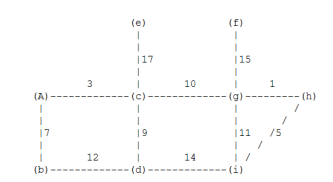
\includegraphics[width=0.5\textwidth]{graph.PNG}
	
	\begin{enumerate}[label=\alph*.)]
		\item \textbf{[5 points]} In what order are edges added to the Minimum Spanning Tree (MST) using
Kruskal's Algorithm? List the edges by giving their endpoints.
		\item \textbf{[5 points]} In what order are edges added to the MST using Prim's Algorithm starting
from vertex A? List the edges by giving their endpoints.
	\end{enumerate}

\solution

\begin{enumerate}[label=\alph*.)]
		\item g-h, A-c, h-i, A-b, c-d, c-g, f-g, c-e
		\item A-c, A-b, c-d, c-g, g-h, h-i, f-g, c-e
	\end{enumerate}
\end{homeworkProblem}

\pagebreak

\begin{homeworkProblem}
	\textbf{[30 points](U \& G Required)} Exercise 22.2-9 (page 602).\\
	\begin{itemize}
		\item[22.2-9)]	Let $G = (V,E)$ be a connected, undirected graph. Give an $\bigo (V + E)$-time algorithm to compute a path in $G$ that traverses each edge in $E$ exactly once in each direction. Describe how you can find your way out of a maze if you are given a large supply of pennies.
	\end{itemize}
\end{homeworkProblem}

\pagebreak

\begin{homeworkProblem}
	\textbf{[30 points](U \& G Required)} Exercise 22.5-6 (page 621).\\
	\begin{itemize}
		\item[22.5-6)]
		Given a directed graph $G = (V,E)$, explain how to create another graph $G'=(V,E')$ such that 
		\begin{enumerate}[label=\alph*.)]
			\item $G'$ has the same strongly connected components as $G$
			\item $G'$ has the same component graph as $G$
			\item $E'$ is as small as possible.
		\end{enumerate}
		Describe a fast algorithm to compute $G'$.			
	\end{itemize}
\end{homeworkProblem}

\pagebreak

\begin{homeworkProblem}
	\textbf{[20 points](U \& G Required)} Exercise 24.3-2 (page 663).\\
	\begin{itemize}
		\item[24.3-2)] Give a simple example of a directed graph with negative-weight edges for which Dijkstra’s algorithm produces incorrect answers. Why doesn’t the proof of Theorem 24.6 go through when negative-weight edges are allowed?					
	\end{itemize}
\end{homeworkProblem}

\pagebreak

\begin{homeworkProblem}[6]
	\textbf{[20 points](Extra Credit)} Exercise 24.3-6 (page 663).\\
	\begin{itemize}
		\item[24.3-6)] We are given a directed graph $G = (V,E)$ on which each edge $(u,v) \in E$ has an associated value $r(u,v)$, which is a rela number in the range $0 \leq r(u,v) \leq 1$ that represents the reliability of a communication channel from vertex $u$ to vertex $v$. We interpret $r(u,v)$ as the probability that the channel from $u$ to $v$ will not fail, and we assume that these probabilities are independent. Give an efficient algorithm to find the most reliable path between two given vertices.
	\end{itemize}
\end{homeworkProblem}

\end{document}